%!TEX root = project.tex

\chapter{System Design}
As many pages as needed.
\begin{itemize}
\item Architecture, UML etc. An overview of the different components of the system. Diagrams etc… Screen shots etc.
\end{itemize}

We aimed to have each player (agent) be capable of observing its own surroundings, so on each frame the agent would be able to make decisions on where it would suit best to move.

Each agent needed to be able to calculate distances relative to itself, such as the distance it is from the ball, the distance it is from its own goal, and the distance it is from the opposition goal [Image1]. 

Also the agent needed to be able to distancing information relating to the closest opponent to itself, such as the distance the closest opponent is to the ball, the distance the closest opponent is from the opposition goal, and the distance the closest opponent is from the agents own goal [Image 2]. 

The overall position of the ball on the pitch would also have to be taken into account, so the agents must have been able to calculate the distance the ball is to the agent's own goal, as well as the distance the ball is to the opposition goal [Image 3]. 

Each agent needed to know what type of player they were, be it a goalkeeper, defender, or striker, and adjust its decision making accordingly, for example, in some scenarios it would be better for a goalkeeper to stay protecting the goals instead of rushing out to challenge the opponent with the ball, however a defender or striker might decide to push forward and challenge the ball in the same scenario, be it there is a goalkeeper positioned in their goals.

Along with each agent knowing which type of player they are, they also need to be able to detect what type of player the closest opposition is, as this could also affect the decision the agent makes, whether the agent should attempt to challenge the ball or if they are better off positioning themselves elsewhere.

Finally, the agent needs to be able to determine the angle the ball sits between themselves and the opposition goals, as well as the angle the ball sits between the agent and their own goal. These angles need to be considered as they will also influence the agent’s decision when moving frame by frame [Image 5].
For example, it would be better for the goalkeeper to position themselves between the ball and the goal here, instead of simply rushing towards the ball and attempting to challenge the opponent [Image 4].

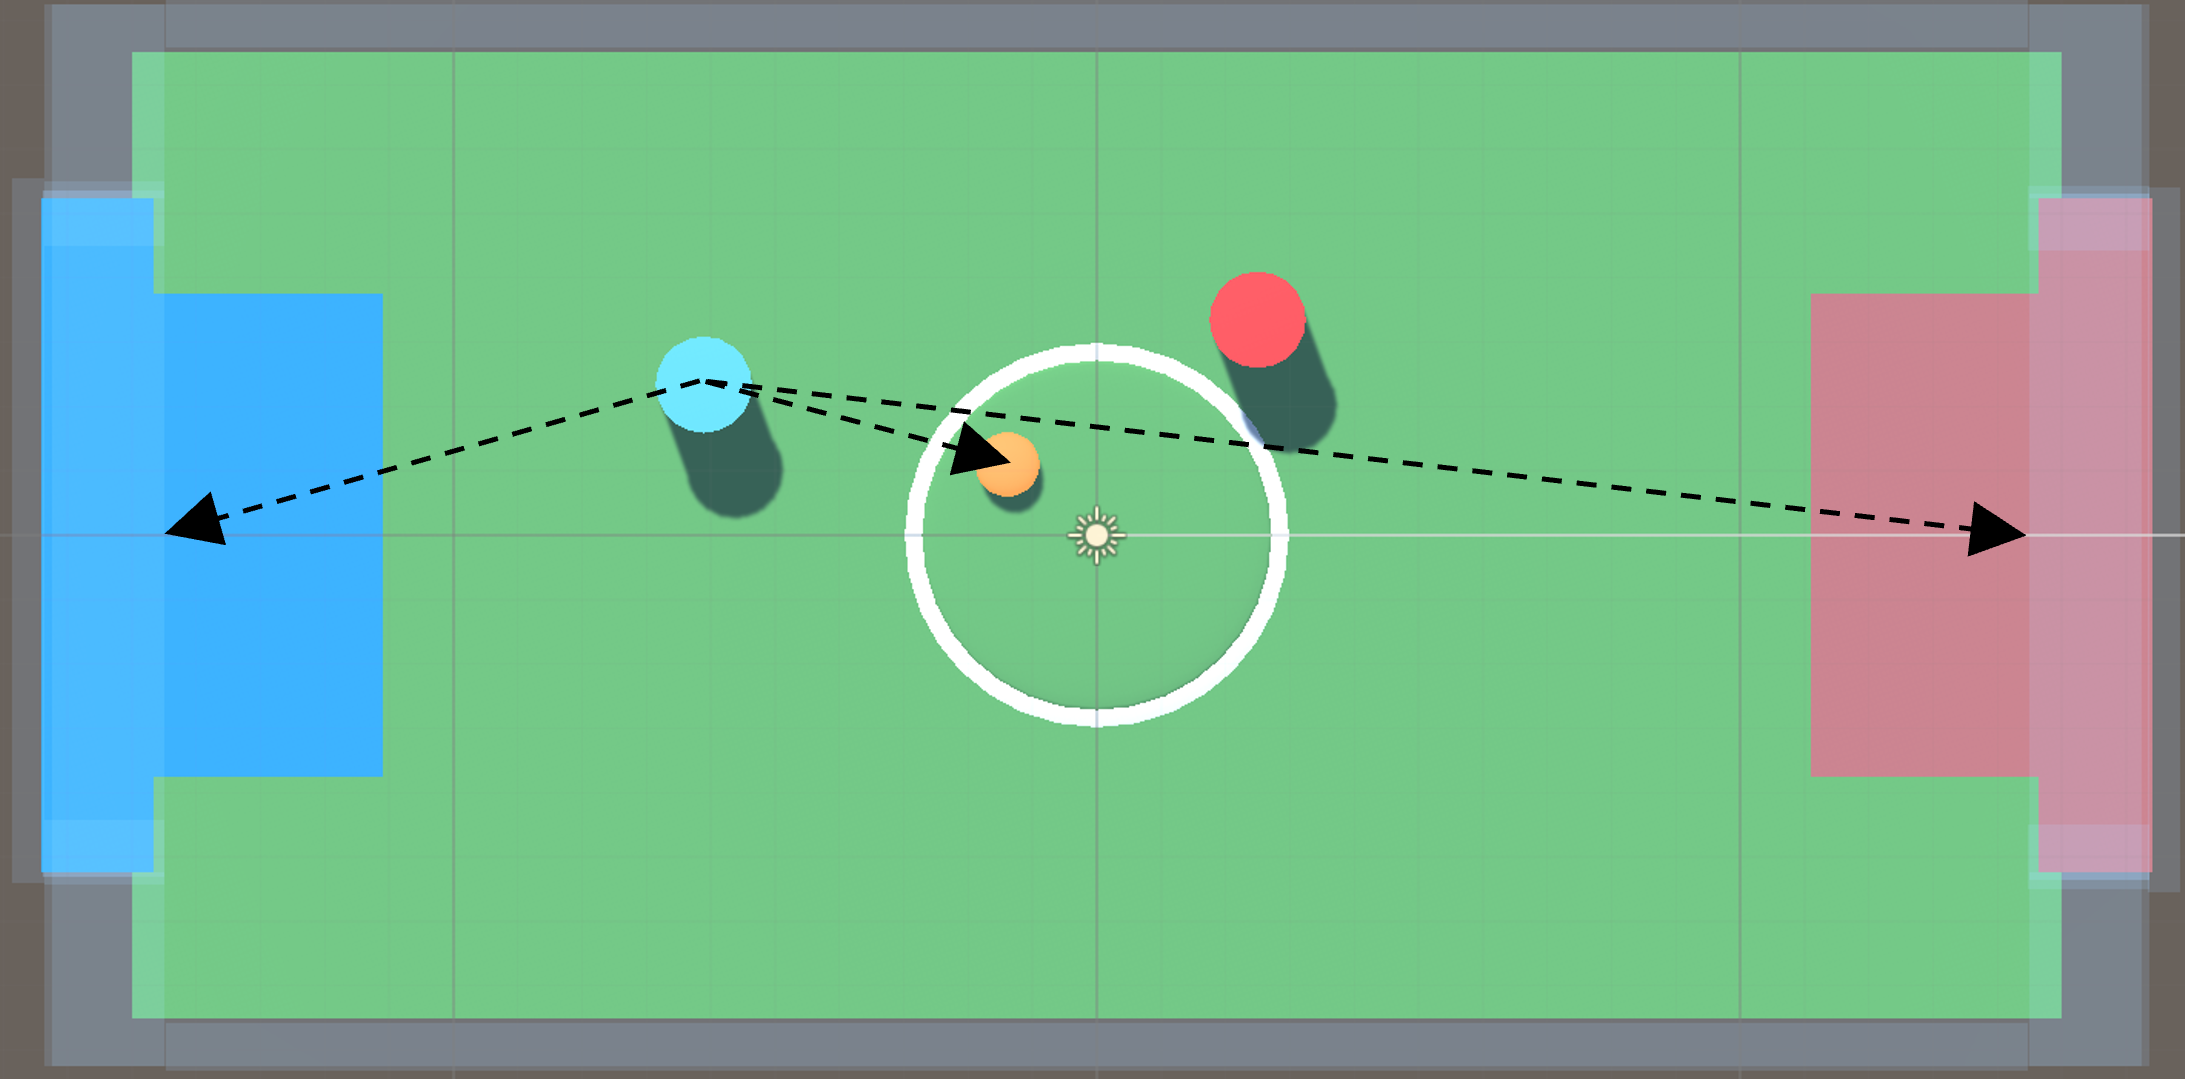
\includegraphics[scale=0.2]{img/Image1.png}


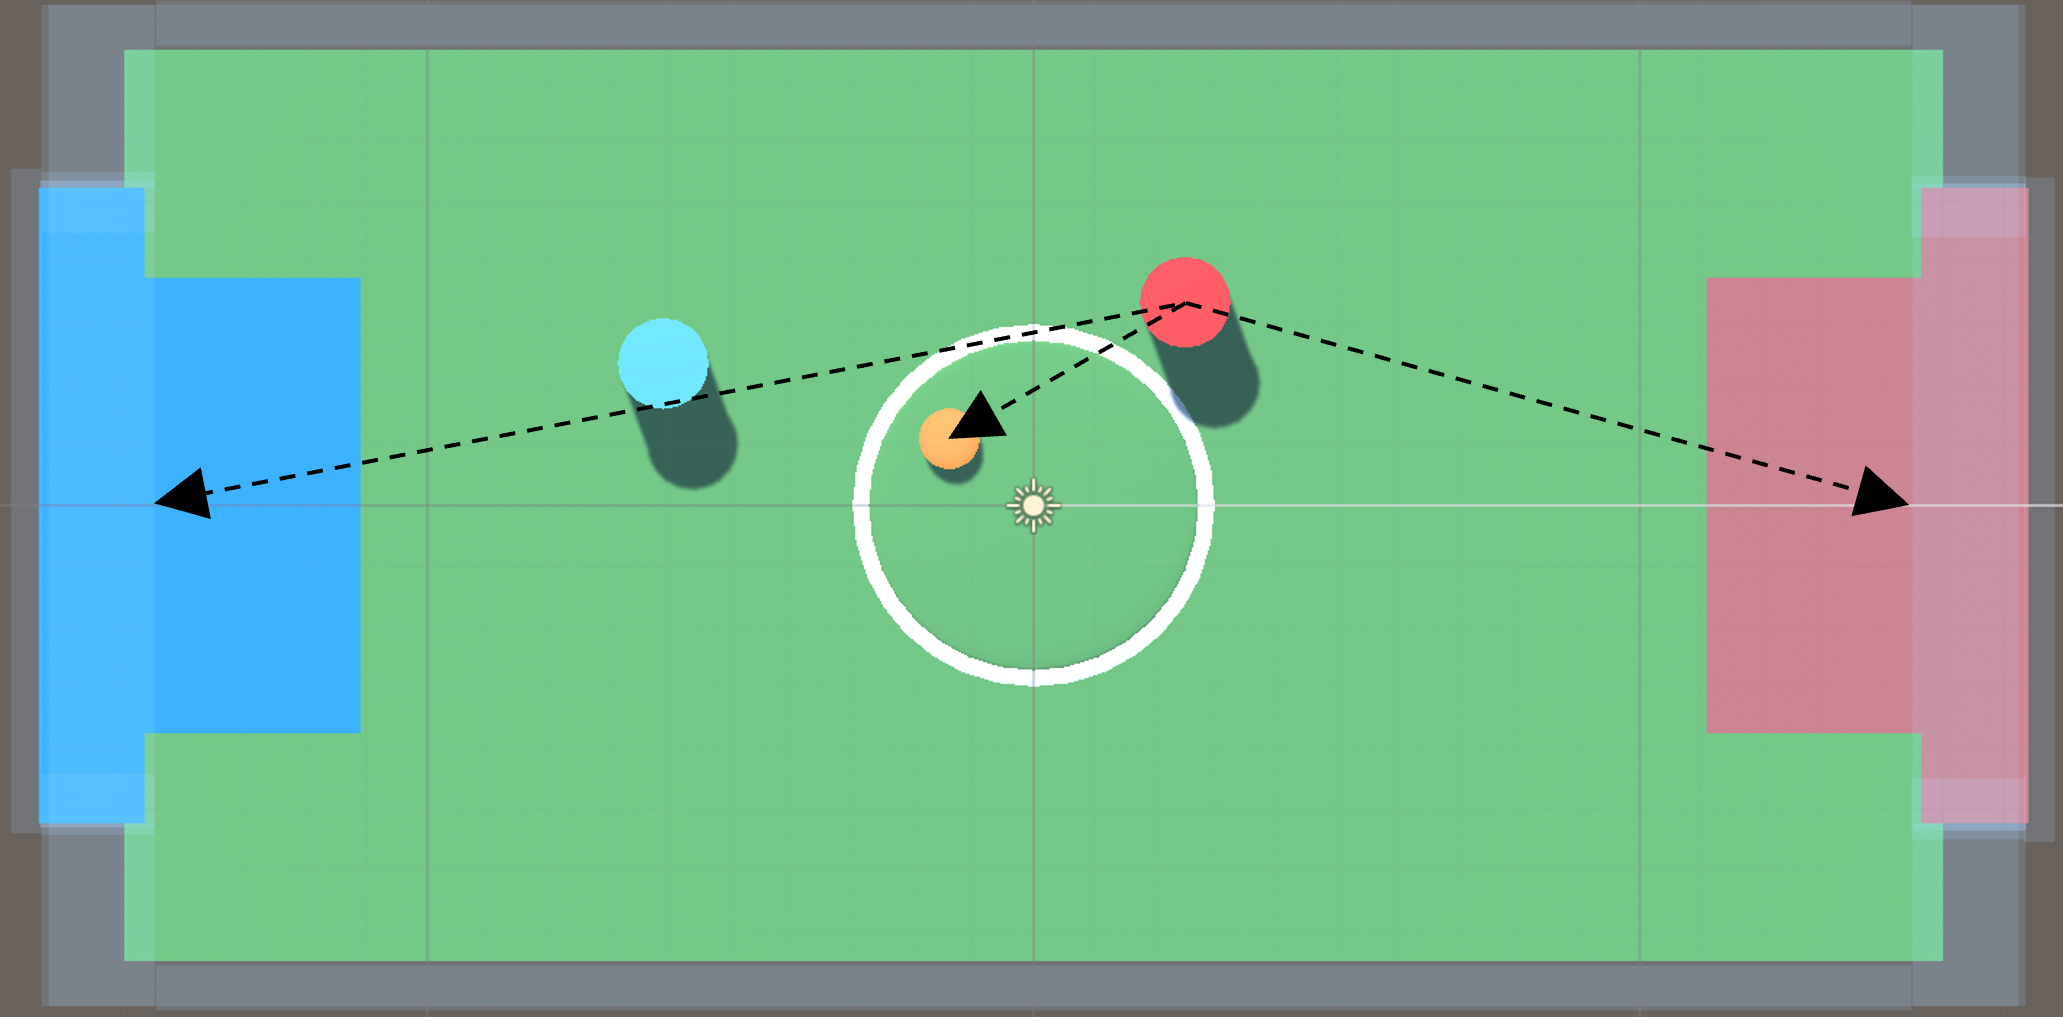
\includegraphics[width=115mm, height=55mm]{img/Image2.png}

\begin{table}[h]
  \centering
  \begin{tabular}{x{2cm}p{3cm}}
    \toprule \\
    Column 1 & Column 2 \\
    \midrule \\
    Rows 2.1 & Row 2.2 \\
    \bottomrule
  \end{tabular}
  \caption{A table.}
  \label{table:mytable}
\end{table}